

\documentclass{beamer}


% Code Including
\usepackage{xcolor}
\usepackage{setspace}
\usepackage{color}
\usepackage{listings}
% Define a custom color
\definecolor{backcolour}{rgb}{18,21,25}
\definecolor{codegreen}{rgb}{0,0.6,0}
\definecolor{blackl}{RGB}{11,12,15}
\definecolor{greyl}{RGB}{18,21,25}

% Define a custom style
\lstdefinestyle{myStyle}{
	backgroundcolor=\color{greyl},   
	commentstyle=\color{codegreen},
	basicstyle=\ttfamily\footnotesize,
	breakatwhitespace=false,         
	breaklines=true,                 
	keepspaces=true,                 
	numbers=left,       
	numbersep=5pt,                  
	showspaces=false,                
	showstringspaces=false,
	showtabs=false,                  
	tabsize=2,
}






\usetheme{Warsaw} %Berkeley Goettingen Hannover Berlin
\setbeamercolor{normal text}{fg=white,bg=blackl}
\setbeamercolor{structure}{fg=white}

\setbeamercolor{alerted text}{fg=red!85!black}

\setbeamercolor{item projected}{use=item,fg=black,bg=item.fg!35}

\setbeamercolor*{palette primary}{use=structure,fg=structure.fg}
\setbeamercolor*{palette secondary}{use=structure,fg=greyl!95!blackl}
\setbeamercolor*{palette tertiary}{use=structure,fg=greyl!90!blackl}
\setbeamercolor*{palette quaternary}{use=structure,fg=structure.fg!95!black,bg=blackl!80}

\setbeamercolor*{framesubtitle}{fg=white}

\setbeamercolor*{block title}{parent=structure,bg=black!60}
\setbeamercolor*{block body}{fg=black,bg=black!10}
\setbeamercolor*{block title alerted}{parent=alerted text,bg=black!15}
\setbeamercolor*{block title example}{parent=example text,bg=black!15}

\usepackage{german}


\begin{document}

\title{OpenCV}   
\author{Florian Herrmann} 
\date{\today}
\logo{
\includegraphics[scale=0.3]{Bilder/HAWK_Logo.jpg}
	
\includegraphics[scale=0.004]{Bilder/Blank.png}
	 
\includegraphics[scale=0.15]{Bilder/OpenCV.png}}

\begin{frame}
\titlepage
\end{frame}

\section{Namensgebung \& Historie}
\begin{frame} \frametitle{Namensgebung}
	$Open + Computer Visson = OpenCV$ 
	\begin{description}
		\item Open:\\
		 Open-Source-Software.
		\item Computer Visson:\\
		 Verschiedene Formen der Detektoren, Filtern und Bildableitungen (+ ML).
	\end{description}
\cite{Bradski2008}
\end{frame}

\begin{frame} \frametitle{Historie}
	\begin{itemize}
		\item [2000] Initiation durch Intel (um mehr Prozessoren zu verkaufen). 
		\item [2013] Die Willow Garage gibt an Itseez ab. 
		\item [2016] Intel kauft Itseez 
	\end{itemize}
	\cite{Bradski2008}
\end{frame}
\section{Funktionen}
\begin{frame} \frametitle{Funktionsumfang}
	\begin{columns}
		\begin{column}{0.5\textwidth}
			\textbf{Klassische Bildverarbeitung: }
			\begin{itemize}
				\item  2 und 3D Merkmallsextraktion.
				\item Klassische Filter.
				\item Gesichts und Gesten erkennen.
				\item Mensch Maschine Interaktion.
				\item Segmentierung.
				\item Klassifizierung.
				\item Steriskopisches Sehen.
				\item Kalman-Filter.
			\end{itemize}
		\end{column}
		\begin{column}{0.5\textwidth}
			\textbf{Maschinelles Lernen:}
			\begin{itemize}
				\item NNK Nächster Nachbar Klassifikation.
				\item Deep Learning.
			\end{itemize}
			\textbf{Tools zur verbesserten Nutzung:}
			\begin{itemize}
				\item GUI zur leichteren Ausgabe von Bildern.
			\end{itemize}
		\end{column}
	\end{columns}	
	\cite{Bradski2008}
\end{frame}

\begin{frame} \frametitle{Maintainer}
	\begin{itemize}
		\item OpenCV ist Opensource $\rightarrow$ Code liegt auf Github.
		\item Unterliegt der Apache Lizenz.
		\item Jeder Kann mit  Pull/Merge-Requests mitarbeiten.
		\item Regelmäßige Teilnahme am: Google Summer of Code
		\item Finaziert durch Crowdfunding
	\end{itemize}
	\begin{figure}
		\centering
		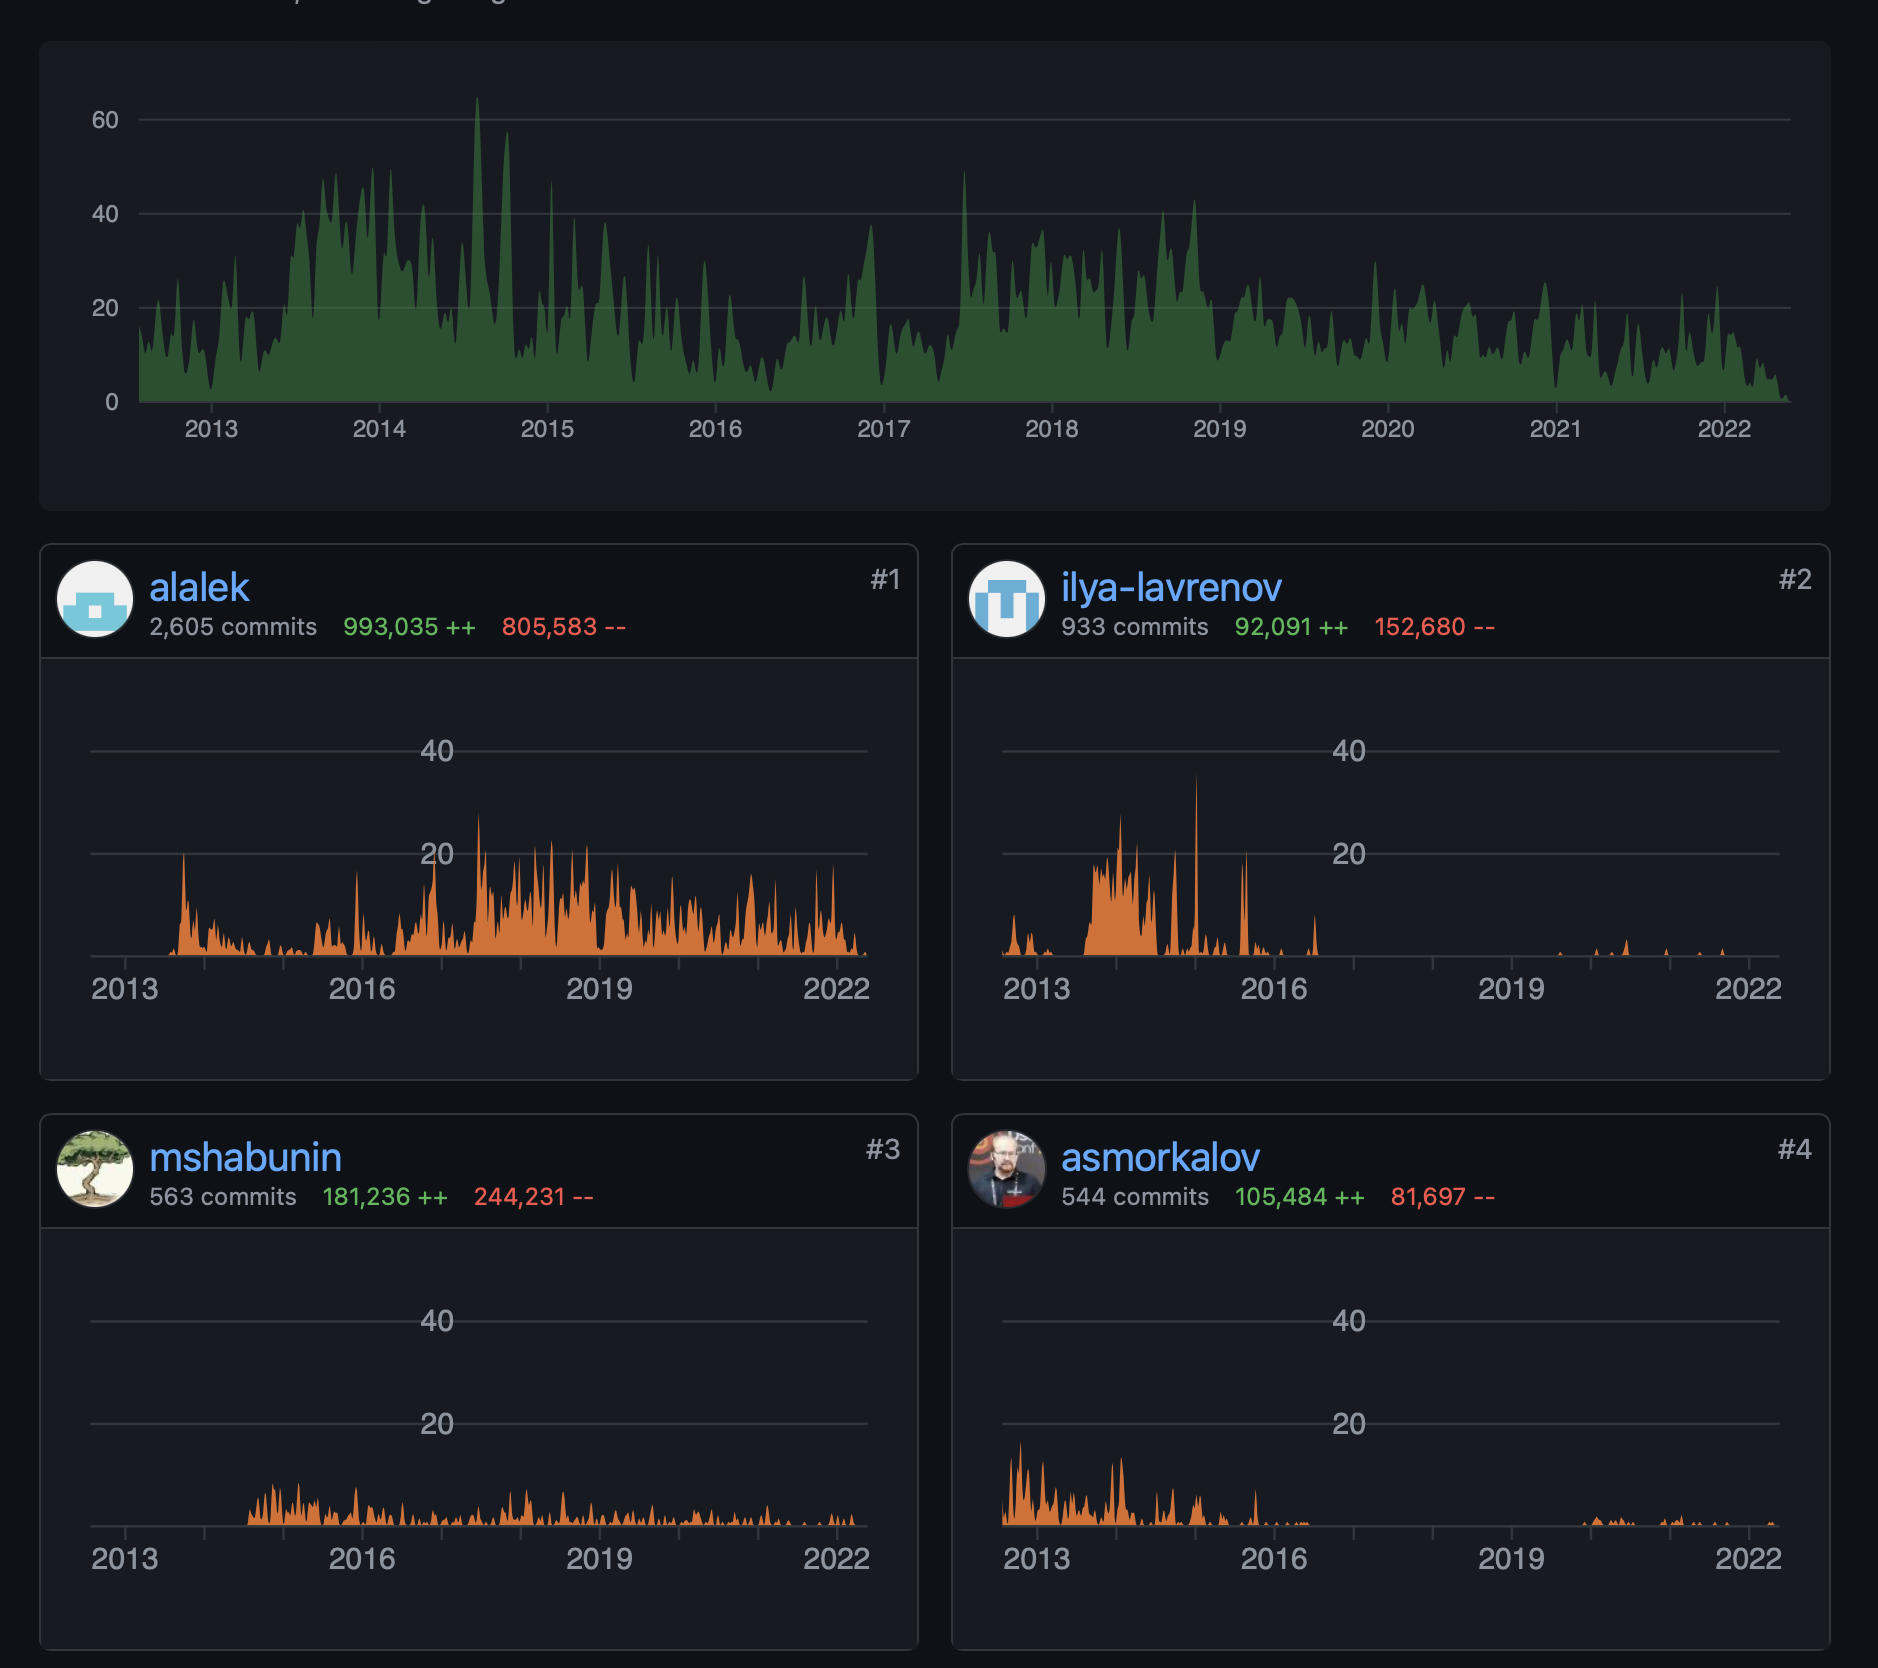
\includegraphics[width=0.5\textwidth]{Bilder/maintainer.png}
		\label{a5}
	\end{figure}
	\cite{GitHub, Bradski2008}
\end{frame}



\begin{frame} \frametitle{Programmierung und Kompatibilität}
	Programiert in C++ (Laufzeit Optimierung, paralleles berechnen).
	\begin{figure}
		\centering
		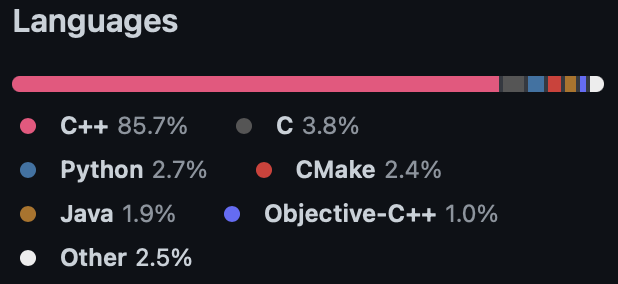
\includegraphics[width=0.8\textwidth]{Bilder/CodeBase.png}
		\label{a4}
	\end{figure}
\cite{GitHub, Bradski2008}
\end{frame}

\section{Kompatibilität}
\begin{frame} \frametitle{Programmierung und Kompatibilität}
\begin{columns}
\begin{column}{0.5\textwidth}
			\textbf{Dabei ist OpenCV kompatibel mit:}
			\begin{itemize}
				\item C
				\item C++
				\item Python
				\item Java
			\end{itemize}
		\textbf{Und ist auf den folgenden Systemen verfügbar:}
		\begin{itemize}
			\item Windows
			\item Mac
			\item Linux
			\item Embedded Systems
		\end{itemize}
	\end{column}


	\begin{column}{0.5\textwidth}
			\centering
			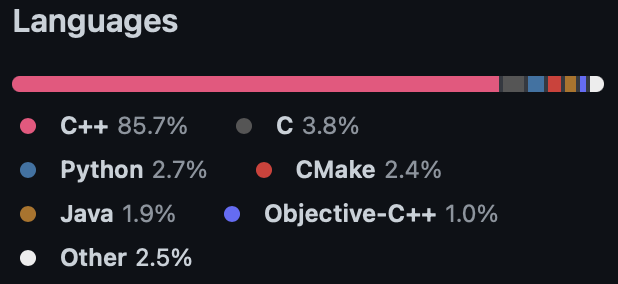
\includegraphics[width=\textwidth]{Bilder/CodeBase.png}
	\end{column}
\end{columns}	
\end{frame}





\section{Installation}
\begin{frame} \frametitle{Hardware Voraussetzungen}
	\textbf{Anforderungen: }
	\begin{itemize}
		\item  min. 4 GB RAM.
		\item Festplattenspeicherbedarf vernachlässigbar klein.  
		\item Hardware Beschleunigung nur mit NVDIA GPU möglich(CUDA).
	\end{itemize}
\end{frame}

\begin{frame} [fragile]
\frametitle{Instalation}
	\textbf{Möglichkeit 1: Selbst kompilieren}\\
	Aufwändig und Vollständig.
		\begin{itemize}
			\item  [1.] git clone https://github.com/opencv/opencv
			\item [2.] cmake opencv
		\end{itemize}
	\textbf{Möglichkeit 2: Installation über eine Pipeline}\\
	Einfach und möglicherweise nicht ganz aktuell.\\
\lstset{style=myStyle}
\begin{lstlisting}
		pip3 install opencv-python 
\end{lstlisting}
\cite{Howse2015}
\end{frame}
\section{Vor-,Nachteile}
\begin{frame} \frametitle{Vor- \& Nachteile}
	\begin{columns}
		\begin{column}{0.5\textwidth}
			\textbf{Vorteile:}
			\begin{itemize}
				\item Auf allen Plattformen verfügbar
				\item Schnelle Berechnungen
				\item Weit verbreitet
				\item Freie Lizenz
				\item Sehr gut dokumentiert
				\item Kompatibel mit anderen Bibliotheken
			\end{itemize}
		\end{column}
		
		
		\begin{column}{0.5\textwidth}
			\textbf{Nachteil:}
			\begin{itemize}
				\item Nicht ganz einfache Nutzung im Vergleich zu GUI Anwendungen
				\item Teilweise aufwendige Installation
			\end{itemize}
		\end{column}
	\end{columns}
\end{frame}

\section{Beispiele (Demo)}
\begin{frame} [fragile]
\frametitle{Beispiele}
	\textbf{Bild öffnen und anzeigen}\\
\lstset{style=myStyle}
	\begin{lstlisting}
	import cv2   as cv								#Lade OpenCV
	
	filename = "example.png". 				#Pfad zum Bild 
	image = cv.imread(filename,0)  		#Bild Laden
	if image is None:               
		print("Unable to open " + filename)
		exit(-1)

	cv.imshow("An example image", image)    #Bild anzeigen
	cv.waitKey(0)
	cv.destroyAllWindows()
	\end{lstlisting}
	\cite{Howse2015}
\end{frame}

\begin{frame} [fragile]
\frametitle{Beispiele}
	\textbf{Kanten Erkennung:}\\
	\lstset{style=myStyle}
	\begin{lstlisting}
		import cv2 as cv
		import numpy as np
		
		image = cv.imread('imge.png',0)
		
		height, width = image.shape
		
		canny = cv.Canny(image, 50, 120)
		cv.imshow('Canny', canny)
		
		cv.destroyAllWindows()
	\end{lstlisting}
	\cite{Howse2015}
\end{frame}

\begin{frame} [fragile]
	\frametitle{Beispiele}
	\textbf{Gesichtserkennung:}\\
	\lstset{style=myStyle}
	\begin{lstlisting}
		import cv2 as cv
		capture = cv.VideoCapture(0)
		cascade = cv.CascadeClassifier("haarcascade_frontalface_default.xml")
		while True:
			_, im = capture.read()
			im_gray = cv.cvtColor(im, cv.COLOR_BGR2GRAY)
			face = cascade.detectMultiScale(im_gray)
			for x, y, width, height in face:
				cv.rectangle(im, (x, y), (x + width, y + height), color = (0,0,250), thickness = 5)
			cv.imshow("Kamera", im)
				if cv.waitKey(1) == ord("q"):
				break
		capture.release()
		cv.destroyAllWindows()
	\end{lstlisting}
	\cite{Howse2015}
\end{frame}

\begin{frame}
	\centering \Large
	\emph{Danke für eure Zeit!}
\end{frame}

\section[Quellen]{Referenzen}

\begin{frame}\frametitle{Quellen \& Literatur}
	\begin{thebibliography}{9}
		\bibitem{GitHub} 
		GitHub: OpenCV
		\\\texttt{Open Source Computer Vision Library}
		\url{https://github.com/opencv/opencv}
		[abgerufen am: 21.05.2022]
		
		\bibitem{OpenCV} 
		Website: OpenCV
		\\texttt{Open Source Computer Vision Library}
		\url{https://opencv.org}
		[abgerufen am: 27.05.2022]
		
		\bibitem{Bradski2008}
		Bradski, A. Learning OpenCV - Computer Vision with the OpenCV Library. (OReilly Media, Inc. ,2008)
		
		\bibitem{Howse2015}Howse OpenCV 3 Blueprints - . (Packt Publishing Ltd,2015)
	\end{thebibliography}
\end{frame}




\end{document}
